% ---
% Capitulo de METODOLOGIA
% ---




\chapter{Metodologia}\label{cap:metodologia}

No âmbito desse estudo, é proposta uma arquitetura para implantação de hospedagem de aplicações para a UNITINS, visando o atendimento das solicitações de hospedagem de projetos em diversas plataformas. Assim, o levantamento de informações consistiu em avaliar um conjunto de requisitos essenciais para apoiar o modelo apresentado.

Para a definição das ferramentas, observou-se os seguintes critérios, sendo eles:  a sua disponibilização de código open source, a flexibilidade no uso e confiabilidade nos resultados, as suas vantagens e desvantagens, a aceitação junto a comunidade científica e a documentação disponível, seja por meio de livros ou artigos publicados ou por contribuições junto a comunidade web.

O processo de definição das ferramentas teve como ponto inicial estar em consonância com atuabilidade do mercado de TI e ter continua contribuição da comunidade web. Sendo assim, o primeiro critério a ser considerado foi como a ferramenta daria suporte às diversas linguagens de programações disponíveis. Outro fator relevante está atrelado a maneira como o produto pode ser adquirido, mais diretamente, ao custo necessário para fazer uso da ferramenta. A premissa é que as mesmas deveriam possuir versão \textit{open source} que  dessem suporte às necessidades da arquitetura proposta.

Dessa forma, alguns requisitos foram considerados na escolha, os pontos citados a seguir nortearam a escolha: 
    \vspace*{0.5cm}

\begin{itemize}
	
	\item Extensibilidade: tomando como fato as rápidas mudanças no cenário tecnológico, a ferramenta deveria poder dar suporte a diferentes linguagens e integrações;
	\item Usabilidade: a ferramenta deveria ser de fácil compreensão e fornecer uma boa experiência ao usuário;
	\item Segurança: é essencial que critérios de segurança sejam inerentes à ferramenta, definição de papéis e usuários.
	
\end{itemize}

    \vspace*{0.5cm}

\section{Materiais Utilizados}

Tomando por base os critérios mencionados acima, utilizou-se as seguintes ferramentas detalhadas na Tabela 2.


\begin{table}[htb]
	    \vspace*{0.5cm}
	
	\centering
	\begin{tabular}{l|c}
		\hline
		\multicolumn{1}{c}{DESCRIÇÃO} & VERSÃO/CONFIGURAÇÃO                                                                                         \\ \hline
		Máquina Física                  & \begin{tabular}[c]{@{}c@{}}Mac OS High Sierra 10.13.4 /\\ i5 2.4Ghz 10 GB RAM 1333 MHz DDR3\end{tabular} \\ \hline
		Oracle VirtualBox               & Versão 5.2.8                                                                                             \\ \hline
		Docker                          &   17.12.0-ce                                                                                                 \\ \hline
		GitHub                          & Git 2.18.0                                                                              \\ \hline
		SonarQube                          &  2.8.1                                           \\ \hline
		Jenkins                          & 2.11.2                                        \\ \hline
		Kubernetes                          & Plugin Jenkins - Minikube Versão 1.11                                           \\ \hline
	\end{tabular}
\label{tab:ferramentas}
\caption{Ferramentas utilizadas}
\end{table}

\begin{itemize}
	    \vspace*{0.5cm}
	
\item VirtualBox: Criação de máquinas virtuais para testes. Disponibilização das máquinas virtuais para execução dos hosts clientes e servidores;
\item GitHub: Versionamento e repositório. Esse serviço receberá os códigos das aplicações dos desenvolvedores;
\item Jenkins: Automatização da execução de tarefas e testes de implantação. O Jenkins será executado em uma máquina virtual com Sistema Operacional Ubuntu 16.04 LTS Linux 64 bits.
\item Docker: Contêineres para armazenamento das aplicações e serviços. O Docker será executado em uma máquina virtual com Sistema Operacional Ubuntu 16.04 LTS Linux 64 bits.
\item Kubernetes: Recurso utilizado para criar nós ou slaves, destinados a dividir o peso de compilação, evitando a sobrecarga no nó master do Jenkins, utilizar-se-á versão Minikube.
\item Sonar: Plugin de análise estatística do \textit{build}, com ele será possível coletar resultado das métricas definidas para resultados.

\end{itemize}

    \vspace*{0.5cm}

\section{Arquitetura Proposta}

Para a implantação e adequação do processo de deploy, visando atender as demandas da UNITINS, bem como estar em consonância com a filosofia DevOps, propôs-se a arquitetura ilustrada na Figura \ref{fig:pipelinejenkins}.
Toda a arquitetura é gerida e orquestrada pelo Ansible desde uma nova mudança no repositório do GitHub até o envio para produção.
\\
\begin{figure}
	\centering
	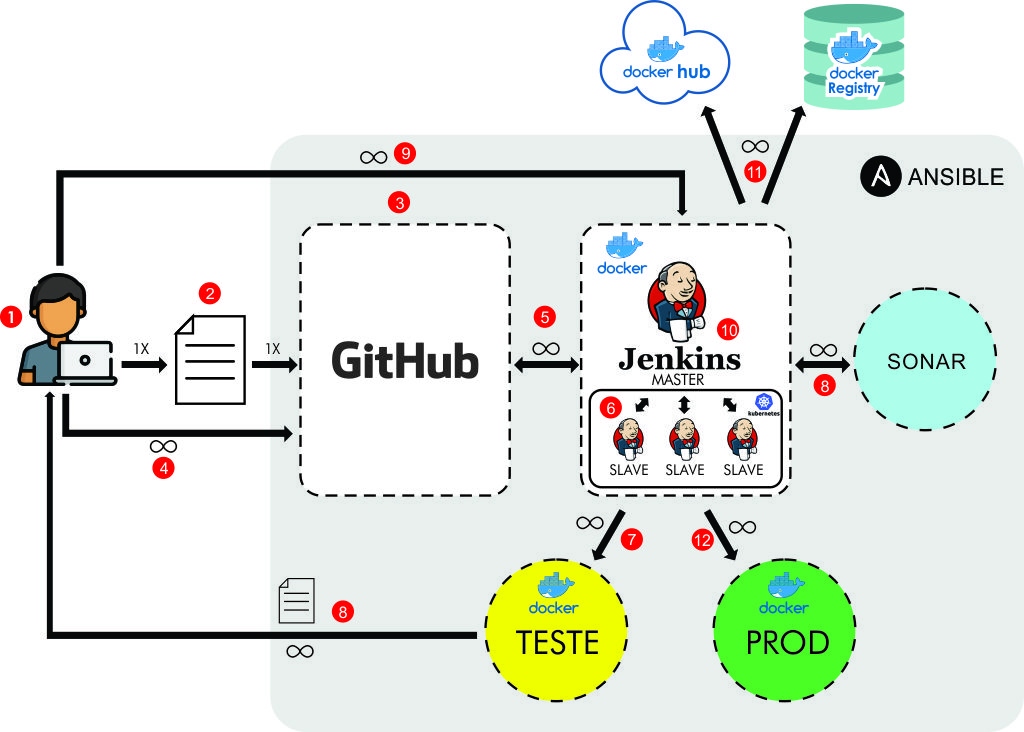
\includegraphics[width=1\linewidth]{imagens/pipelinejenkins}
	\caption{Representação da Arquitetura Proposta}
Fonte: Acervo próprio
\label{fig:pipelinejenkins}
\end{figure}


Considerando o modelo apresentado, pontua-se cada etapa a fim de detalhar o fluxo da disponibilização ao usuário final. O simbolo de infinito representado no na mesma figura, indica que o fluxo nesse ponto é contínuo e se repete a cada nova interação.

\begin{enumerate}
	\item No ponto de partida, é pre-requisito a existência de conteúdo codificado em linguagem de programação, que permita o versionamento do projeto.
	\item O desenvolvedor faz a requisição de um novo ambiente através de formulário web, que contenha as informações pertinentes, tais como link do repositório, dependências do projeto e informações de acesso à aplicação.
	\item A requisição é recebida pelo provedor que verifica os dados de solicitação, avalia a disponibilidade de repositório;
	\item O desenvolvedor envia os commits e o GitHub gera uma notificação de alteração ao Jenkins;
	\item Jenkins recebe a notificação (Git Fetch – Git Merge – Dry Run – Commit Check);
	\item O Jenkins cria instâncias diferentes para construir o projeto, para isso, faz uso do Kubernetes;
	\item O Jenkins incia o \textit{build} e realiza testes automatizados;
	\item O gestor é notificado quanto aos logs e status do \textit{build};
	\item O gestor homologa ou não o \textit{build};
	\item Jenkins gera novo \textit{release} e nova tag de versão;
\item O Ansible informa ao Docker para construir uma nova imagem da aplicação e a envia para um repositório de imagens local, sendo ainda possível o envio para um repositório em numem, como o Docker Hub\footnote{Disponível em: https://hub.docker.com}
	\item Estando as alterações aprovadas o Jenkins através do Ansible realiza deploy da aplicação em um contêiner Docker destinado a produção;
\end{enumerate}

O processo é reiniciado com a chamada de uma nova requisição do código-fonte do aplicativo do repositório Github em questão. Após isso faz-se a atualização da versão do projeto levando-se em conta o número de compilação, assim tem-se uma identificação digital específica para essa implantação.
    \vspace*{0.5cm}

\section{Descrição do Serviço de Integração Contínua}

A fim de criar uma plataforma que possibilitasse a construção e configuração de um ambiente replicável, auto escalável e ágil, foi utilizado o conceito da infraestrutura como código, ou \textit{"as-a-code"}. Nesse sentido, vislumbrou-se um serviço que reunisse as ferramentas Docker, Jenkins e Kubernetes sob orquestração do Ansible para realizar a execução do processo de deploy bem como o provisionamento do ambiente com a instalação dos serviços, dependências e configurações com a chamada do arquivo \textit{Dockerfile} que faz a instalação das dependências para o ambiente Jenkins, bem como as chaves de acesso, instalação de plugins, busca por jobs, e criação dos devidos contêineres Docker. 

A primeira etapa deste processo consiste na disponibilização do  \textit{Formulário de Solicitação de Ambiente de Desenvolvimento (FAD)}, no qual o usuário sinalizará a pretensão de alocação de sua aplicação em servidor web na infraestrutura da UNITINS. Os dados informados nesse formulário gerarão um arquivo \textit{.json} que será lido pela API do Jenkins a fim de se criar um novo \textit{Job} para esse repositório, essa etapa será mais detalhada na subseção \ref{subsection:pipebuild}.

Os arquivos fundamentais desse projeto são primeiramente o \textit{playbook }(cd.yml) do Ansible, ele é responsável por fazer a instalação do Docker e baixar a imagem Jenkins, e então iniciar o processo de configuração do ambiente chamando o \textit{Dockerfile} mencionado anteriormente.

A imagem do Jenkins foi construída com o objetivo da mesma ser replicável e auto-escalável, isso quer dizer que a mesma possui configurações genéricas e, portanto, aplicável em qualquer tarefa a ser executada, sendo os \textit{Playbooks }Ansible de cada serviço responsável por suprir as dependências de cada projeto não disponíveis no Jenkins.

O arquivo \textit{Dockerfile} traz o \textit{script} utilizado para construir as imagens Docker e mapear os volumes externos utilizados pelo Jenkins, como arquivos de configuração e base de dados, além disso esse arquivo inicia os contêineres dos serviços com o comando "run". O arquivo \textit{plugins.txt}\footnote{vide Apêndice A} mapeado para um desses volumes traz uma lista de plugins que serão instalados em tempo de execução no \textit{build} da imagem, assim o Ansible somente instalará plugins mencionados no formulário e que não conste nessa lista, nesse caso é realizado um novo \textit{build} da imagem para atualizar a lista de plugins e/ou demais configurações.

Na raiz do projeto estão os arquivos de configuração do Jenkins. Nesses, estarão os parâmetros necessários para iniciar o serviço do Jenkins sem a necessidade de reconfigurar toda a ferramenta ao reinicio de cada instância. Essa forma de configuração torna o serviço reaproveitável, ou seja, tanto é possível criar um padrão inicial definido para demais projetos do Jenkins, quanto utilizá-lo para execução dos mais diversos tipos de\textit{ jobs}, desde o mais básico ao mais complexo, alocando somente o recurso necessário para cada iteração. Dessa forma, não se desperdiça recurso computacional para os builds mais simples e utilizam-se instâncias diferentes do Jenkins através de \textit{slaves} orquestrados pelo Kubernetes para construções que demandam mais poder computacional.
    \vspace*{0.5cm}

\subsection{Pipeline do Build}\label{subsection:pipebuild}

Para início do processo de \textit{build} do código, é necessário antes de tudo que esteja disponível um repositório de versionamento de códigos, definido aqui com a plataforma do GitHub. Essa sinalização será concebida por meio de um \textit{FAD}. Esse formulário será disponibilizado por um endereço web, onde é premissa que o usuário já possua um repositório para o projeto no GitHub, e preencha os demais campos solicitados do formulário. É requerido desde o nome do responsável pelo projeto até as dependências necessária para execução do mesmo. Essa busca pelos Jobs são feitas pela API do Jenkins semelhantemente ao REST.

Nesse sentido a API pode ser usada para:

\begin{itemize}
	\item Recuperar informações de Jenkins para consumo programático;
	\item Desencadear uma nova compilação;
	\item Criar ou copiar Jobs.
\end{itemize}


O \textit{Pipeline }de um projeto baseia-se num fluxo iniciado na alteração do estado do código-fonte em um repositório até a disponibilização do software em produção. Esse processo tem por natureza um fluxo contínuo da cadeia de comandos da Integração Contínua. Iniciando, o Jenkins é responsável por monitorar o repositório GitHub a fim de verificar alteração no estado do código do projeto utilizando recurso de \textit{Push Notification} já próprio da ferramenta, ou seja, se houveram \textit{commits} no mesmo, o Jenkins atualiza a versão do projeto de acordo com o número de compilação, dessa forma garantisse uma assinatura única da construção durante o processo de implantação. Após atualizar a versão do código partiremos para a construção do mesmo.

Tendo sucesso na compilação, partiremos para a construção do projeto. Após o Jenkins identificar uma alteração no código, o mesmo clona o projeto do repositório, e escalona diferentes estâncias desse mesmo serviço, fazendo o papel de \textit{slaves} e o \textit{master} faz o papel de orquestrador, esse processo retira o peso e custo computacional, se o projeto fosse compilado somente em uma instância master do Jenkins, assim o \textit{build} é distribuído entre os \textit{slaves} e ao final do processo realiza o \textit{merge} do projeto, esse processo é gerenciado pelo \textit{Kubernetes}, utilizando sua versão \textit{Minikube}.

Parte-se então para os testes da aplicação, nesse ponto o fluxo funciona de forma que testes automatizados sejam aplicados e na incidência de erros o Jenkins dispara uma notificação via email para o usuário, ou gestor da equipe de desenvolvimento, informando a causa da falha e o respectivo \textit{log}, caso contrário se os testes lograrem sucesso o Ansible recebe o \textit{build} do Jenkins e realiza o depósito em um ambiente de homologação com Docker. Simultaneamente a isso o gestor do projeto é notificado sobre o sucesso da construção e solicita que o mesmo acesse esse ambiente para a devida homologação.

Sendo aprovada as alterações realizadas, o gestor libera a nova versão para ambiente de produção, então o Jenkins recebe a confirmação e sinaliza ao Ansible que solicitará ao Docker a construção de uma nova imagem da aplicação e exportará a mesma para o Docker Hub onde ficará armazena em repositório na nuvem (é também possível fazer essa guarda e versinamento em repositório local) e então é realizado o \textit{deploy} da imagem em ambiente de produção e iniciado um contêiner do mesma, a partir dai o software já está disponível para acesso pelo usuário final, caso ocorra erro no \textit{deploy} o gestor é notificado. Esse fluxo pode ser mais claramente entendido na representação da Figura \ref{fig:pipelinebuild}.

\begin{figure}[htb]
	\centering
	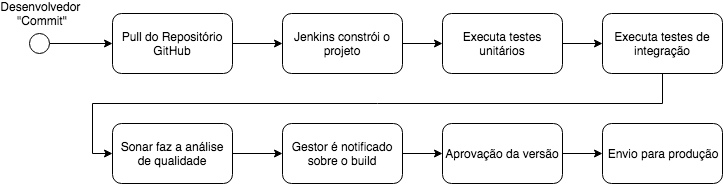
\includegraphics[width=1\linewidth]{imagens/pipelinebuild}
	\caption{Pipeline do Build}
	\label{fig:pipelinebuild}
\end{figure}


Durante todo o processo o SonarQube realiza o monitoramento e coleta dos resultados obtidos em todas as etapas do \textit{deploy}, ao fim do processo é possível verificar nesse ambiente as estatísticas, tomando por base as métricas definidas. Isso dará uma visão mais próxima no que tange o desempenho e qualidade do deploy da aplicação.

\section{Pseudo-códigos dos Algoritmos Implementados}

De maneira a organizar o pipeline do processo de criação dos \textit{jobs }e \textit{build} do código, os \textit{playbooks} foram agrupados por categorias, sendo o \textit{playbook cd.yml} o responsável pela chamada dos demais. Cada Playbook é constituído por diversas funções que identificam o tipo da dependência ou serviço, sua versão, se existe repositório específico ou se o Ansible fará a gestão deste, e a definição da \textit{tag} que identifica a qual serviço essa função pertence.

A partir do momento que o ambiente é provisionado pelo Ansible, o pipeline é refeito utilizando os \textit{playbooks} de \textit{Jobs} para atualização de novos projetos, e \textit{Builds} para construção do código já atribuído a um \textit{Job}.

    \vspace*{2cm}
O Algoritmo 1 faz menção a execução do playbook inicial do Ansible, nele será solicitado a execução de cada um dos demais playbooks que dizem respeito aos serviços necessário para o ambiente:

\begin{algorithm}[H]
	\SetAlgoLined
	\Entrada{\textit{Playbook Ansible}} 
	\Saida{Chamada de demais Playbooks Ansible}
	\Inicio{
			execute o playbook java \\
			execute o playbook docker \\
			execute o playbook registry \\
			execute o playbook jenkins	\\					  
	}
	\Retorna{Ambiente provisionado}
	\label{alg:algoritmo01}
	\caption{\textsc{Provisionamento de Ambiente}}
\end{algorithm}
\newpage 
O Algoritmo 2 trata da execução de cada playbook de serviço, onde verifica-se cada função que trata as dependências exigidas para que esse serviço possa funcionar:

\begin{algorithm}[H]
	\SetAlgoLined
	\Entrada{\textit{Playbook }de cada serviço} 
	
	\Saida{Instalação dos serviços utilizando configurações genéricas}
	
	\Inicio{
		\Para{cada função}	{
		defina o nome da função \\
		defina o nome do serviço \\
		\Se{possuir repositório específico}{
			repositório $\gets$ url
		}
		defina a tag que identifica a função
	}
	execute todas as funções					  
	}
	\Retorna{Instalação de serviço}
	\label{alg:algoritmo02}
	\caption{\textsc{Instalação de serviço}}
\end{algorithm}

    \vspace*{2cm}
O Algoritmo 3 busca por Jobs em um diretório mapeado pelo contêiner Docker de cada serviço, nesse diretório serão armazenados os arquivos .json gerados com o preenchimento do formulário de solicitação de ambiente de desenvolvimento:	

\begin{algorithm}[H]
	\SetAlgoLined
	\Entrada{Arquivo \textit{Json}} 
	
	\Saida{\textit{Job}}
		diretorioDosJobs: string\\
		jobs:lista
	
	\Inicio{
		\Se{\textit{Jobs não estiver vazio}} {
			\Para{\textit{cada json}}{
			leia o arquivo \textit{Json}\\
			novoJob $\gets$ adicioneBuild(json)			
		}
		}				  
	}
	\Retorna{\textit{Jobs}}
	\label{alg:algoritmo03}
	\caption{\textsc{Jobs - Funcionalidade: Busca por Jobs}}
\end{algorithm}

    
O Algoritmo 4 trata da execução dos Jobs no Jenkins, onde passa pela busca de jobs no diretório, baixa o código do repositório git informado no formulário, gera uma nova versão do código e se autorizado pelo gestor, executa o contêiner:	

\begin{algorithm}[H]
	\SetAlgoLined
	\Entrada{Playbook de \textit{Build} e \textit{Job}} 
	\Saida{Criação do Job e execução do contêiner}
	
	\Inicio{
			  \Para{\textit{cada novo Job}}{
			  Execute o Dockerfile\\
			  Defina o diretório de alocação do Job\\
			  Baixe o código fonte do repositório\\
			  Compile o código\\
			  \Se{\textit{não houver erros}}{
			  		construa imagem Docker da aplicação\\
			  		faça upload da nova imagem para o Registry\\
			  		solicite revisão do gestor\\
			  		\Se{\textit{autorizado}}{
			  			Baixe a nova imagem Docker\\
			  			Execute o contêiner da imagem\\
		  			}
		  		}
	  		\Senao{
	  			Envie email ao responsável do projeto
  			}
		  }
	}

	\label{alg:algoritmo04}
	\caption{\textsc{Ansible - Jenkins - Docker: \textit{Build} e \textit{Job}}}
\end{algorithm}



    \pagebreak[4]
\section{Métricas}

A definição de mecanismos que forneçam e possibilitem a análise estatística de todo o processo é fundamental dentro deste projeto. Nesse sentido, o uso de métricas se faz necessário para que se tenha uma visão próxima de cada processo de \textit{deploy}. Assim, adota-se neste trabalho, as seguintes métricas detalhas na Tabela ??.


\begin{table}[h]
	\small
	\begin{tabular}{l|c}
		\hline
		\multicolumn{1}{c|}{MÉTRICA} & DESCRIÇÃO \\ \hline
		Tempo de Deploy & \begin{tabular}[c]{@{}c@{}}Critério utilizado para avaliar o tempo gasto para\\ uma atualização de aplicação entrar em produção\end{tabular} \\ \hline
		Taxa de erros & Ocorrência de erros retornados durante a execução\\dos Jobs. \\ \hline
		\begin{tabular}[c]{@{}l@{}}Desempenho frente a múltiplos\\ deploys\end{tabular} & \begin{tabular}[c]{@{}c@{}}Medição do desempenho obtido frente\\ à um estresse de deploys simultâneos\end{tabular} \\ \hline
		\begin{tabular}[c]{@{}l@{}}Recurso computacional \\consumido utilizando diferentes\\instâncias de Slaves.\end{tabular} & \begin{tabular}[c]{@{}c@{}}Quantidade de recursos de memória e processamento\\utilizados entre os slaves para concluir a tarefa iniciada.\end{tabular} \\ \hline
	\end{tabular}
\label{table:metricas}
\caption{Métricas Definidas}
\end{table}


Os resultados das métricas definidas são importantes pois com isso é possível ter noção muito próxima da "saúde" do código, pontos de fragilidade, potenciais melhorias, eventuais de melhorias nos recursos físicos e previsão de tempo de entrega de uma funcionalidade. Esses pontos dão suporte para tomadas de decisões por parte do gestor do projeto. Em se tratando do SonarQube a própria ferramenta já traz uma série de métricas pré-definidas e genéricas que podem ser aplicadas aos mais diversos tipos de jobs, e nesse ponto é importante ressaltar que é possível a criação de \textit{scripts} específicos de testes de acordo com o tipo de tarefa que está sendo executada no \textit{build}, no entanto o foco aqui não foi a implementação dos testes, mas sim a provisão do ambiente de automatização.
